\chapter{Methodology}
\label{methodology}
In the previous chapters, extensive details over the parameterization of the wing surface, CFD solver, and niching algorithms are covered. This chapter deals with the flow of data from the initial step of creating NACA 0012 airfoil as baseline geometry to the end that is obtaining the optimized wing surfaces. More emphasis is given on the implementation of the FFD box, SVD method, use of glyph script for meshing in pointwise, use of SU2 solver, and way to submit jobs into the cluster. Figure \ref{cp_flowchart} represents the flowchart mentioning the steps involved in obtaining perturbed control points. Every segment in the flowchart will be explained in detail in the subsequent sections.

% Define block styles

\tikzstyle{block} = [rectangle, draw, fill=blue!20, 
text width=25em, text centered, rounded corners, minimum height=3em]
\tikzstyle{line} = [draw, -latex']
\tikzstyle{block1} = [rectangle, draw, fill=blue!20, 
text width=25em, text centered, minimum height=3em]

\begin{figure}
  \centering
  \begin{tikzpicture}[node distance = 2.5cm, auto]
    % nodes
    \node [block] (init) {\Large NACA equation with cosine function};
    \node [block1, below of = init] (new1) {\Large NACA airfoil (*.x3d)};
    \node [block1, below of = new1] (inte) {\Large Wing surface generation (baseline wing)};
    \node [block1, below of = inte] (inte2) {\Large FFD box over the baseline wing};
    \node [block1, below of = inte2] (inte3) {\Large FFD box corner control points};
    \node [block1, below of = inte3] (inte4) {\Large Interpolation of the FFD corner points};
    \node [block1, below of = inte4] (final) {\Large Cartesian coordinates of all control points (*.csv)};
    \node [block, below of = final] (continue) {\Large Continue ...};
   
    % edges
    \path [line] (init) -- node {\Large python script} (new1);
    \path [line] (new1) -- node {\Large extrude in span direction} (inte);
    \path [line] (inte) -- node {\Large glyph script} (inte2);
    \path [line] (inte2) -- node {\Large outcome } (inte3) ;
    \path [line] (inte3) -- node {\Large python script} (inte4) ;
    \path [line] (inte4) -- node {\Large outcome} (final) ;
    \path [line] (final) -- (continue) ;
  \end{tikzpicture}
  \caption{Flowchart representing the steps involved in generating the perturbed control points}
  \label{cp_flowchart}
\end{figure}


\section{Generation of NACA0012 wing surface}
This work starts with creating the baseline NACA0012 airfoil using standard equations and extruding it in the third dimension to get the wing surface. The detailed steps involved in this process are explained here.

Constructing the NACA four digit airfoils starts with finding the camber line distance ($y_c$), and the thickness ($y_t$) of airfoil upper and lower surfaces
from the chord line. After that appending both the values to get the coordinates of the upper and lower surfaces of the airfoil. Since the airfoil of interest is symmetric, both the camber line and chord line coincide, resulting in $y_c$ equal to zero.
    

Equation \ref{2D_airfoil_thickness} represents the formula to obtain the half-thickness of symmetric NACA four-digits airfoil.
\begin{equation}
y_{t}=5 t\left[0.2969 \sqrt{x}-0.1260 x-0.3516 x^{2}+0.2843 x^{3}-0.1015 x^{4}\right]
\label{2D_airfoil_thickness}
\end{equation}
where,\\
$x$ is position along the chord from 0 to 1.\\
$y_t$ is the half thickness for a given $x$.\\
$t$ is the maximum thickness represented in terms of chord.

Equation \ref{2D_airfoil_thickness} will result in the blunt airfoil at the trailing edge. If a sharp trailing edge is required, one of the coefficients should be modified to zero their sum. Modifying the last coefficient to $-0.1036$ will result in a small change in the overall shape of the airfoil, and a sharp trailing edge is obtained. 

Let ($x_U$, $y_U$), and ($x_L$, $y_L$) presents the upper and the lower airfoil surface coordinates respectively. Since the airfoil is symmetric, $y_c$ is equal zero.
This results in the airfoil coordinates as shown in equation \ref{2d_final_points}.
\begin{equation}
\begin{array}{ll}
x_{U}=x & y_{U}= +y_{t} \\
x_{L}=x & y_{L}= -y_{t}
\end{array}
\label{2d_final_points}
\end{equation}



Considering all the above equation; a Python script is constructed to obtain airfoil coordinates, and the outcome is represented in figure \ref{uniform_points_airfoil}.
\begin{figure}[!htbp]
    \centering
    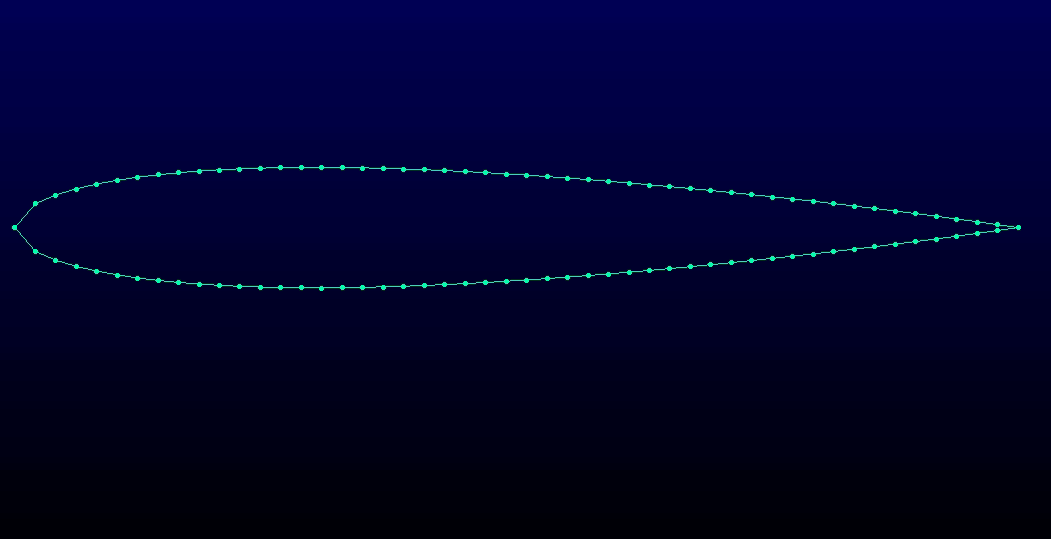
\includegraphics[scale = 0.4]{figures/airfoil_uniform_points.png}
    \caption{Uniform distribution of points along horizontal direction [total 100 grid points].}
    \label{uniform_points_airfoil}
\end{figure}

From figure \ref{uniform_points_airfoil}, it can be noted that the distribution of grid points is uniform from leading edge to trailing edge. However, this will result in incorrect results of pressure distribution while performing CFD simulation. To obtain a good mesh where more points are clustered at the leading edge, cosine function (equation \ref{cosine_function}) is used, instead of the linear distribution of grid points. Figure \ref{cosine_points_airfoil} represent the cosine functional distribution of grid points in horizontal directions.
\begin{equation}
    \begin{array}{l}
        x = 1 - \cos{\theta}  \\
        \forall  \theta \in \left(0, \frac{\pi}{2}\right)
    \end{array}
\label{cosine_function}
\end{equation}

\begin{figure}[!htbp]
    \centering
    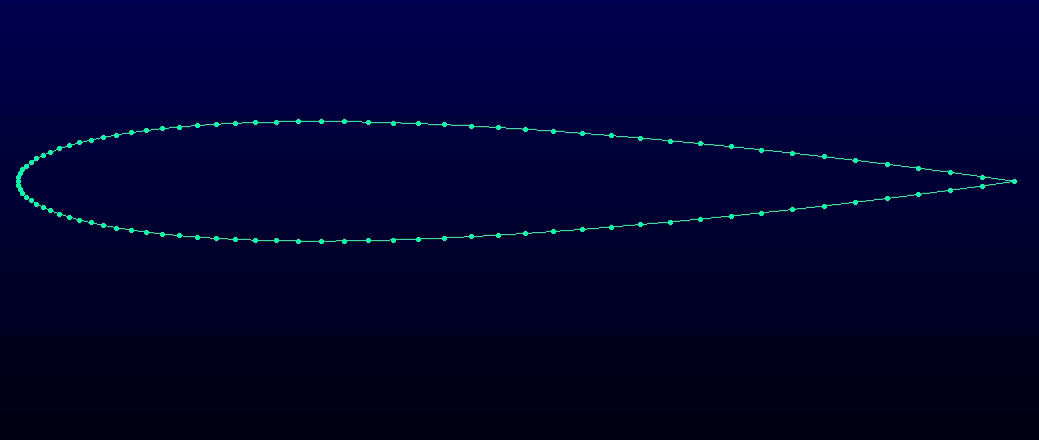
\includegraphics[scale = 0.4]{figures/airfoil_cosine.png}
    \caption{Cosine function distribution of points along horizontal direction [total 100 grid points].}
    \label{cosine_points_airfoil}
\end{figure}

Further, the cosine functional airfoil data is imported into pointwise (meshing software) in the Plot3D (*.x3d) format. Plot3D format is chosen because of the ease of readability. Other formats can also be opted based on convenience. In this work, grid points of 300 along the chord direction are used. Further, the obtained airfoil is extruded (normal extrusion) for three units (1 unit = 1 chord length) in the third dimension (span direction), resulting in the NACA0012 wing mesh. Based on the grid sensitivity analysis, a mesh point of 200 is used along the span direction. Figure (\ref{naca0012 wing mesh}) represents the outcome of spanwise extrusion. This wing surface is a reference (baseline surface), and this work focuses on optimizing the obtained wing shape. 

\begin{figure}
    \centering
    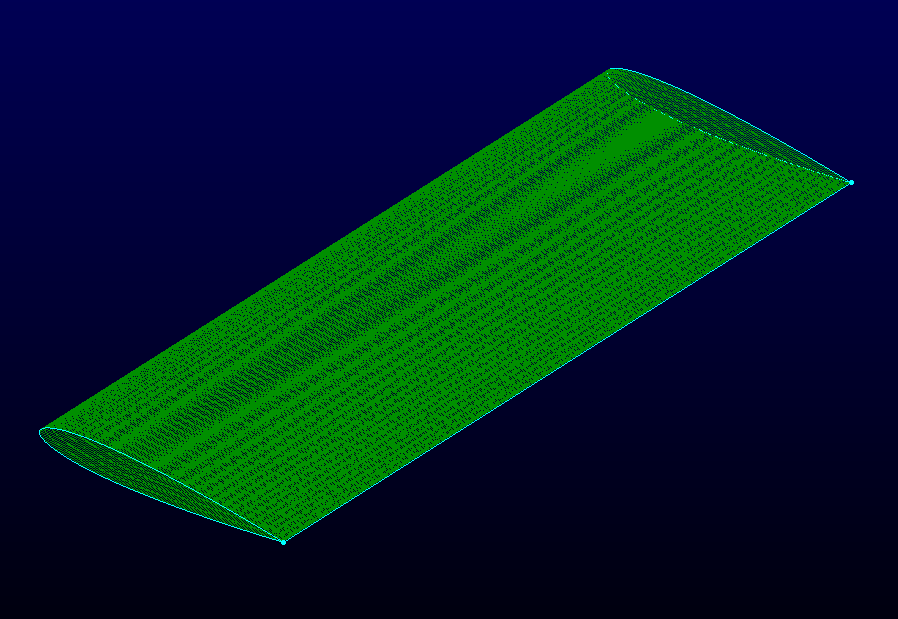
\includegraphics[height=59mm, width=\textwidth]{figures/wing_3d.png}
    \caption{NACA0012 surface mesh (300 $\times$ 200) grid points.}
    \label{naca0012 wing mesh}
\end{figure}


\section{FFD box over baseline mesh}
\begin{figure}
    \centering
    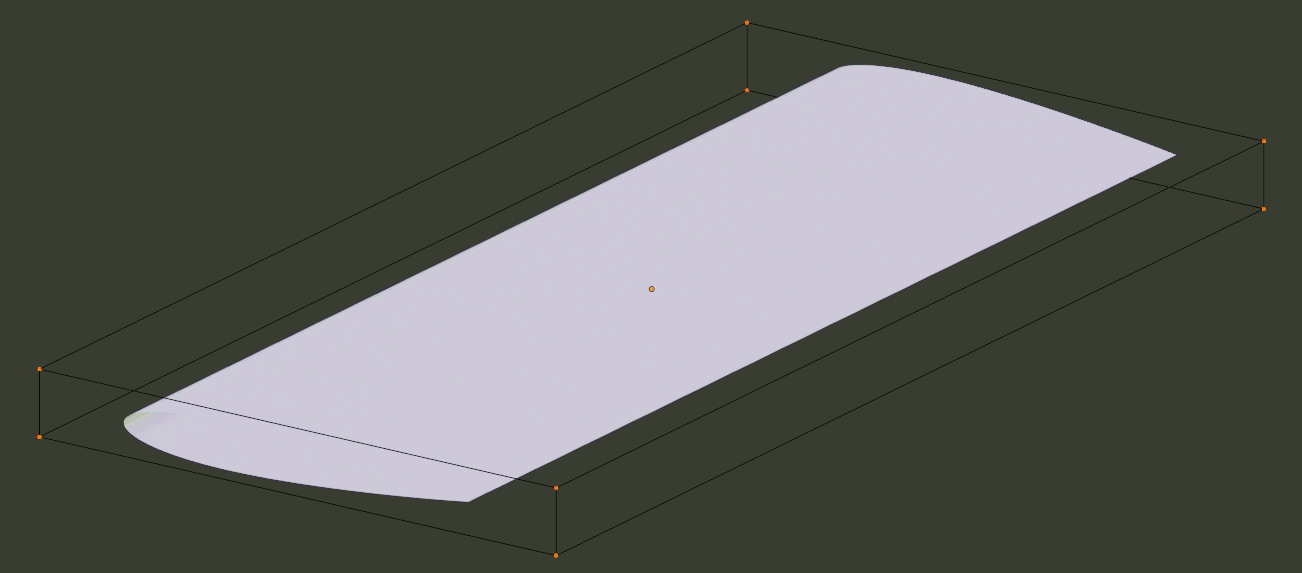
\includegraphics[height = 70mm, width=\textwidth]{figures/wing_FFD_corner_pt.png}
    \caption{FFD box coupled with NACA0012 wing surface. Corner points highlighted act as control points.}
    \label{ffd_wing_corner}
\end{figure}
After obtaining the baseline wing mesh, the FFD box or lattice needs to be covered over the surface where deformation is required. In this work, the entire wing surface is subject of interest. Hence, the whole body is covered with the FFD box. The FFD can either be constructed using the available GitHub code or by manually noting down the extreme ends of mesh and adding the scale factor to the coordinates points. In this work, code in glyph script is used to get the FFD box coordinates points. Here, the scale factor of 1.5 times the chord's length is used along the chord direction. The 50$\%$ higher value of scale factor is used because the nearer the FFD control points, higher will be their influence over the object in interest. To reduce the influence and have higher tolerance (design space), an additional scale factor is used. In the same line, a scale factor of 1.1 is used along the thickness direction, and 1 unit along span direction is used. Figure \ref{ffd_wing_corner} represents the wing surface being circumvented by the FFD box. The highlighted points (corner points) represents the control points of the FFD box. From figure \ref{ffd_wing_corner}, it is observed that the control points in the chord direction are 25$\%$ away from the extreme ends of the wing shape. Finally, the FFD box of size $1.5 \times 0.14 \times 3$ $(chord \times thickness \times span)$ units is obtained. 

\section{Interpolating FFD box control points}
In figure \ref{ffd_wing_corner}, there are a total of eight control points (active control points), and each control point can be displaced in XYZ space independently. This results in a total of 24 (8 $\times$ 3) independent perturbation in a given space. In other words, the dimension of the problem becomes 24. However, in figure \ref{sphere_ffd}, eight control points were circumventing the sphere. The effect of perturbing right top corner point resulting in sphere shape perturbation. The effect of perturbation follows Bernstein polynomial (equation \ref{bernstein_poly}), and the effect is always surrounded near to the perturbed control point (figure \ref{ffd_effect}).

Furthermore, to get a required shape, a higher displacement of control points will be necessary. To solve this issue and to distribute the effect of control points perturbation over an object, more control points have to spread over the subject of interest. There are several ways to add more control points, like log scale distribution, radial distribution, to name a few. However, the simplest one is considered a linear distribution of additional control points between the corner control points. 

A python script is constructed, which takes corner points coordinates, the number of additional points required as input, and result in intermediate control points coordinates as output. Figure \ref{ffd_wing_interpolate} represents the corner control points along with intermediate control points. In this work, there are a total of five control points along chord direction, two along the thickness direction, and six control points along span direction. In total, there are 60 control points, or 180 effective points available for perturbation. Now, the dimension of the problem is 180 (60 $\times$ 3).    
\begin{figure}
    \centering
    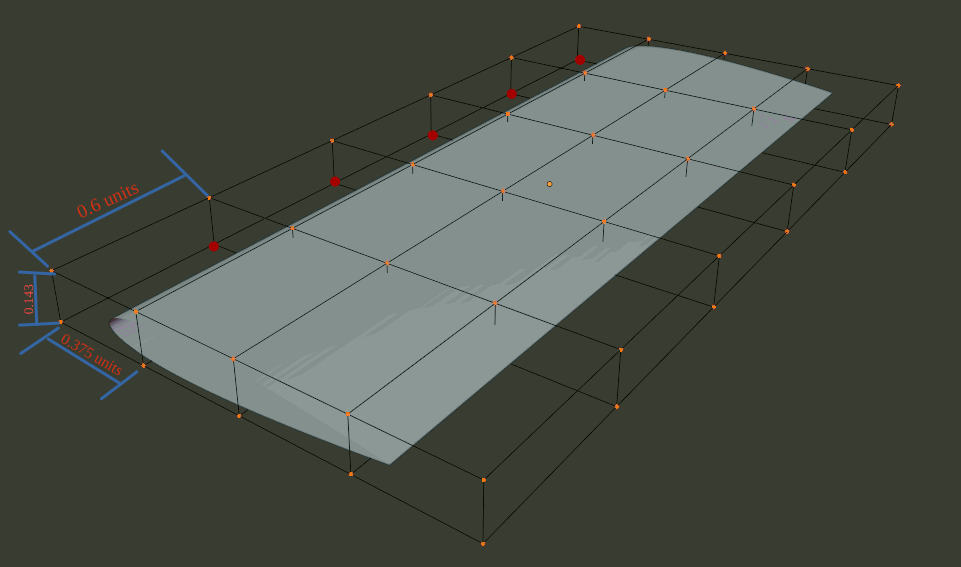
\includegraphics[height = 70mm, width=\textwidth]{figures/wing_all_cp_FFD.png}
    \caption{FFD box along with interpolated points and corner points.}
    \label{ffd_wing_interpolate}
\end{figure}

\section{Control points perturbation}
After placing the desired number of control points over the wing surface, the wing surface mesh points need to be parameterized for the FFD box. This implies the cartesian coordinates of wing surface mesh points will be mapped into parametric form $(X, Y, Z)$ to $(s,t,u)$. This is because once the control points are perturbed, the cartesian coordinates $x,y,z$ of a given point converts to $x_1$, $y_1$, $z_1$. However, the given point's parametric form remains the same as $s,t,u$. This is the crucial step in implementing the FFD box method for parameterizing the wing surface. For any $i^{th}$ surface mesh point, the parametric form can be represented using the equation \ref{parameter_equation}.

\begin{equation}
\begin{array}{lll}
s_i = \frac{x_i - x_{origin}}{\Delta x}, & t_i = \frac{y_i - y_{origin}}{\Delta y}, & u_i = \frac{z_i - z_{origin}}{\Delta z} 
\end{array}
\label{parameter_equation}
\end{equation}

where,\\
$s_i$, $t_i$, $u_i$ are the parametric form of $i^{th}$ mesh point. \\
$x_i$, $y_i$, $z_i$ are the cartesian form of $i^{th}$ mesh point. \\
$x_{origin}$, $y_{origin}$, $z_{origin}$ are the cartesian coordinates of the selected FFD box corner point. \\
$\Delta x$ , $\Delta y$, $\Delta z$ are the differences between extreme points coordinates in the FFD box.\\

\begin{figure}
    \centering
    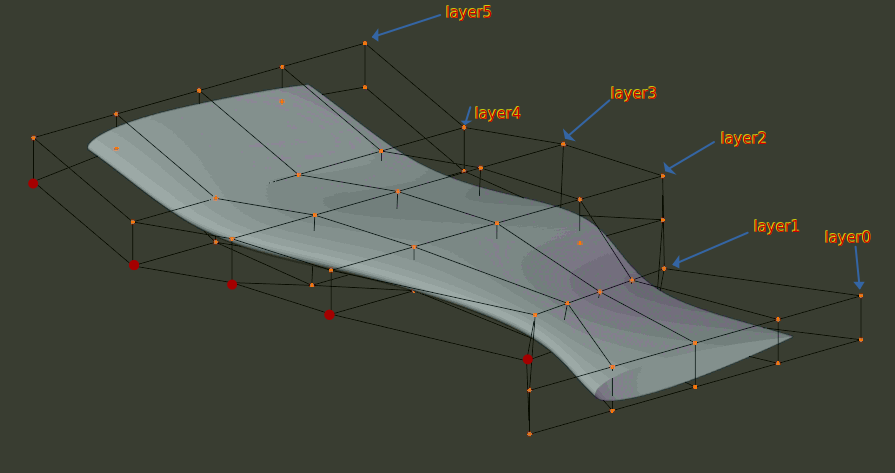
\includegraphics[height = 70mm, width=\textwidth]{figures/wing_FFD-_displaced.png}
    \caption{Effect of control points perturbation on the wing surface.}
    \label{ffd_box_perturbed}
\end{figure}
Now, the entire wing mesh points are mapped to parametric space. After this, perturbating any point of the FFD will lead to an object's shape deformation. For example, consider the entire FFD control points to be divided into layers along the span direction. Layer 0 is located at the wing root section, layer 1 at 0.6 units away from the root section,$ \dots $, and layer 5 at the wing tip section. From figure \ref{ffd_box_perturbed}, layer 1 is contracted from all directions resulting in thickness and chord reduction. Similarly, layer 2 is slightly uplifted, which shows the sign of an anhedral effect. Other layers can also be perturbed similarly to obtain different behaviors towards airflow.

It should be noted that each control point can be perturbed independently, resulting in camber airfoil properties in some sections along the span direction. The choice in the number of layers is user-dependent. However, a choice of lower layers of the FFD along span direction would not be sufficient to obtain multimodality. Similarly, it is applicable in chord direction too. However, a two FFD point in thickness direction would be sufficient because the thickness length is insignificant over the chord and span direction length of the wing. In this work, a polynomial function of order five, four, linear will fit in the span, chord, and thickness direction respectively.

It is observed that allowing all control points will result in complete shape deformation. In some cases, the wing shapes could be infeasible. For example, the perturbed wing could possess a higher slender ratio, or the upper surface and the lower surface of the wing may intersect each other. Avoiding infeasible wing shape is possible by providing proper tolerance (design space) to all control points. Along with this, even some of the control points movement need to be restricted in a particular direction. 

In the present work, the control points at the wing root section are restricted in the chord and thickness direction only. In other words, the control points in layer 0 can perturb in chord and thickness direction and no perturbation in span direction resulting in a reduction of the dimension by 10. Also, the control points from layer 1 to layer 5 can perturb by the same values in the span direction. For example, all control points in layer1 can perturb by the same value (say 0.2) in span direction. A similar approach is carried to layer 2, 3,  and 5. With this, there will be a further reduction in the dimension by 45 (5 layers $\times$ 9 values). In total, dimension of problem is reduced by 55. By the end of this process, the dimension will be 125 (180 - 55). In other words, 125 values are required to define a wing. 

After fixing the dimension (125), design space (tolerance for each dimension) must be sensibly selected. If higher design space is selected, the intersection of the upper and lower wing surface will occur. On the other hand, selecting a lower design space may not result in multimodality. 

As mentioned before, there are five, two, and six control points in this work, along with chord, thickness, and span directions, respectively. A scale factor of 1.5 is selected along the chord direction. Therefore, the distance between subsequent control points along the chord direction is 0.375 units (1 unit = 1 chord length). At maximum, the control points along the chord direction can perturb by the value, which is half the distance between them, that is $\leq$ 0.1875 units. Similarly, along the thickness direction, a control point can perturb by value $\leq$ 0.07 units. Along the span direction, it will be $\leq$ 0.3 units. 

A .csv file $(design space.csv)$ containing design space vectors in 60 rows and 3 columns is created. The point in which perturbation is limited to specific direction contains positive values, whereas those points whose movement is not allowed in a particular direction are set to zero. It can be observed that along the thickness direction, not much design space is available for optimization.

Consider figure \ref{ffd_wing_interpolate}, there are total 6 layers along the span directions (layer 0 to layer 5). The control point represented with red dot acts as a leading control point in that particular layer. During generating a wing, a leading control point is initially perturbed along thickness direction by the value $ \pm $0.25 about the initial coordinate point (leading point coordinate corresponding to initial baseline wing). Further, the remaining lower control points (four in number) in that layer are perturbed by value $\pm$0.1 about the perturbed leading control point coordinate. The upper control points in that layer are perturbed between the corresponding lower control point coordinate and 0.2 above it (lower control point + 0.2). Following this tedious process, it is possible to obtain the curvilinear (of order 5) wing shape along the span direction. Performing this step will guarantee additional design space, which also results in enhancing the possibility of obtaining the multimodality. The following lines represent the upper and lower limits (box constraint) of the design space in all possible dimensions (individuals).

\begin{enumerate}
\item Along chord direction: All control points (60 in number) are allowed to perturb by 0.1875 about their initial coordinate value (control point coordinate representing baseline geometry).
\item Along span direction: Except root section control points, all other control points are allowed to perturb by value 0.3.
\item Along thickness direction: 
\begin{itemize}
\item Leading control point of a layer is perturbed by value  $\pm$ 0.25 about the initial FFD control point coordinate.
\item Lower control points in that layer are perturbed by value $\pm$ 0.1 about leading control point coordinate.
\item Upper control points in that layer are perturbed between the corresponding lower control point and 0.2 higher than it.  
\item Same process is repeated to all remaining layers along span direction.
\end{itemize}
\end{enumerate}

\begin{figure}
    \centering
    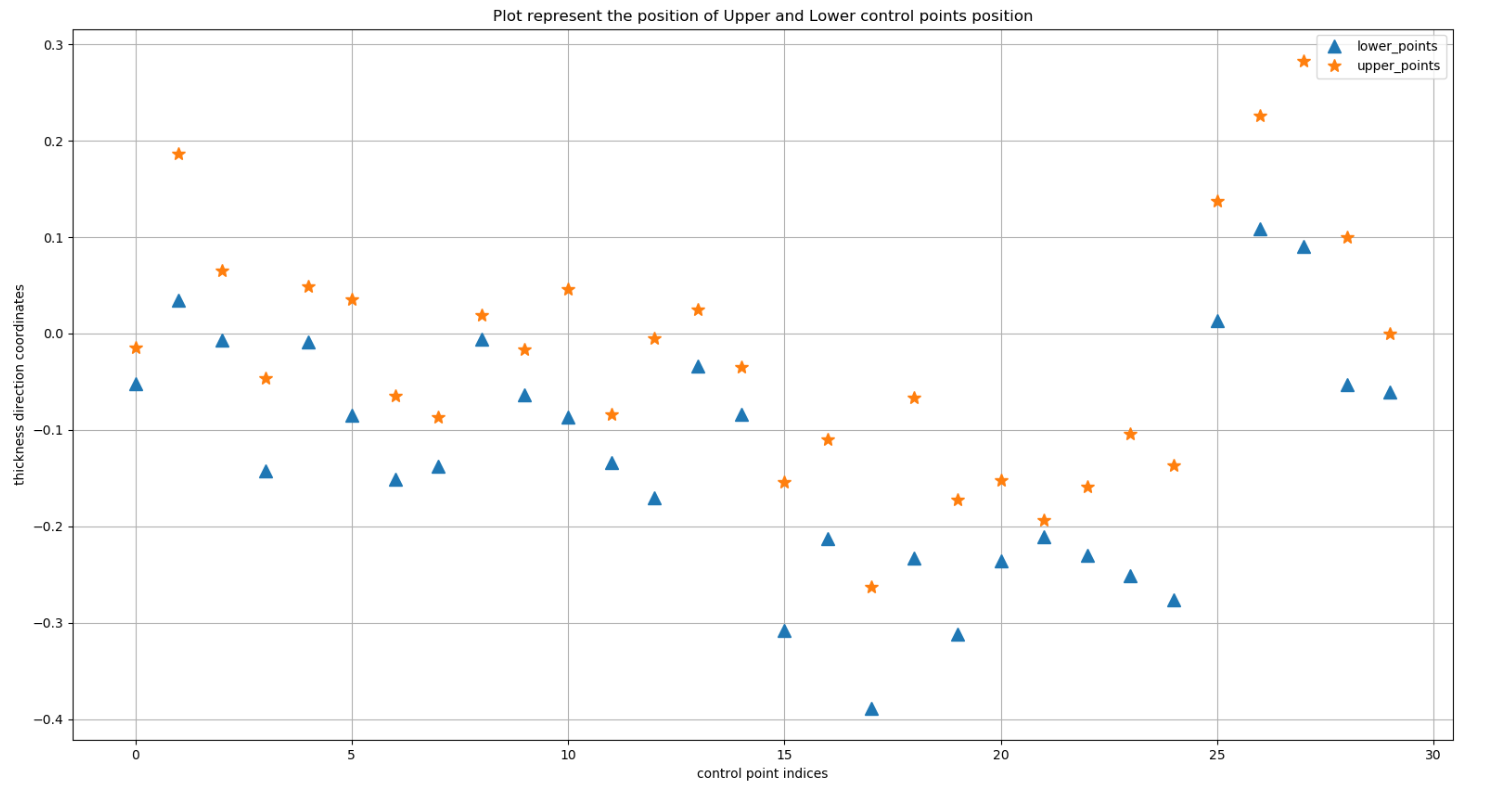
\includegraphics[width=\textwidth, height=70mm]{figures/thickness_direction_plot.png}
    \caption{Plot representing distribution of control points in thickness direction.}
    \label{thickness_plot_control_point}
\end{figure}

A plot representing the control point position in the thickness direction is shown in figure \ref{thickness_plot_control_point}. Y-axis represents the thickness direction position of control points. The X-axis represents the indices of control points. Index 0 to 4 corresponds to layer 0 control points; index 5-9 represent the layer one control points, and so on. The plot shows that for a given wing, the upper control points are always positioned above the corresponding lower control points. This indicates that the wing upper surface will not intersect with the lower wing surface. Also, as mentioned before, the upper control point is at a distance of $\leq$ 0.2 above the corresponding lower control point.


% Define block styles

\tikzstyle{block} = [rectangle, draw, fill=blue!20, text centered, rounded corners, text width=10em]
\tikzstyle{line} = [draw, -latex']
\tikzstyle{block1} = [rectangle, draw, fill=blue!20, text centered, text width=10em]
\tikzstyle{block12} = [trapezium, trapezium left angle=70, trapezium right angle=110, text centered, draw=black, fill=blue!20, text width=10em]

\begin{figure}
  \centering
  \begin{tikzpicture}[node distance = 2cm, auto]
    % nodes
    \node [block] (continue) {\Large Continued ...};
    \node [block12, below of = continue] (parameter) {\large Parametric baseline wing};
    \node [block12, right of = parameter, node distance = 7cm] (cp_new) {\large Perturbed control points};
    \node [block1, below of= parameter, node distance = 2cm] (ffd_box) {\large FFD box equation};
    \node [block, below of= ffd_box, node distance = 2cm] (final) {\large Perturbed cartesian wing coordinates};
    
    % edges
    \path [line] (continue) -- (parameter);
    \path [line] (continue) -| (cp_new);
    \path [line] (parameter) -- (ffd_box);
    \path [line] (cp_new) |- (ffd_box);
    \path [line] (ffd_box) -- (final);
  \end{tikzpicture}
  \caption{Block diagram representing the input and output to FFD box equation.}
  \label{ffd_diagram}
\end{figure}

After completing the design space choice, perturbed control points coordinates are chosen between the respective allowable design space. Further, the parametric form of baseline wing and the new perturbed control points are passed as input to the FFD box equation \ref{ffd_3d}. Here, by considering new control points coordinates, a new set of cartesian coordinates of the perturbed wing is obtained as output. A block diagram representing the same is as shown (figure \ref{ffd_diagram}). Further details about the FFD box equation are explained in chapter \ref{parameterization}.

\section{Implementing PCA}
With 125 design variables defining the feasible design space will satisfy the geometric constraints. Now, it is planned to reduce the dimension representing the design space. However, by using a lower dimension (reduced-order modelling) to represent the design space will not cover the entire design space. Furthermore, by perturbing each design variables with a narrow range, it is possible to obtain the feasible design space. Also, for optimization, the DE algorithm is implemented given geometric constraints. The DE algorithms are not tested for the problem with a dimension greater than 30. There is a need to reduce the problem dimension, which can be achieved by implementing the PCA. 

Initially, the sample space containing perturbed wings needs to be constructed. For example, let $N$ be the number of perturbed wings being generated within the design space. It should be noted that, the range for each of these design variable (125) is the same as mentioned in the previous section. In this work, based on the literature survey and computational power available, a generation cycle of 50 and a population size of 20 is chosen, resulting in the total CFD calculation (functional evaluation) of 1000 $(50 \times 20)$. Based on experience, $N=1000$ perturbed wings are generated. It is possible to generate a large number of the perturbed wings. But, this will create issues while calculating SVD. Each of these wing coordinates $(x_1, y_1, z_1, x_2, y_2, ...,x_n, y_n, z_n)$ are arranged in a row. Also, each wing is defined by $n=30000$ grid points resulting in a matrix (S) of size $1000 \times 90000$. In other words, this is defined as $N$ samples having $n$ features.

Mathematically, let the coordinates of baseline geometry be defined by p coordinated points $x_{i}^{0}$ $\in$ $\mathbb{R}^{m}$, $i=1, \ldots, p$,  where m represents the data's dimension. Also, let n sets of measurements 
$\left\{\hat{x}_{i, j} \in \mathbb{R}^{m} \mid i=1, \ldots, p\right\} ; j=1, \ldots, n$ be available. Here index $j$ refers to a specific instance of measurement, and index $i$ refers to measurements representing a unique nominal coordinate point.

Later, the error matrix is calculated by taking the difference between the $S$ matrix and baseline vector (NACA0012 wing) $B$. The resultant matrix is subtracted from the average error vector, resulting in a covariance matrix $C_x$. Subject the covariance matrix $C_x$ for Singular Value Decomposition (SVD) calculation. There are builtin package available in python to calculate SVD. The outcome of SVD is three matrices $U, \Sigma, V^T$. The matrix $U$ is of size $1000 \times 1000$, $\Sigma$ is a diagonal matrix of size $1000 \times 1000$, and the matrix $V^T$ is of size $1000 \times 90000$. Mathematically,

The error from the nominal geometry is given as,
$$x_{i, j}^{\prime}=\hat{x}_{i, j}-x_{i}^{0}$$

Further, subtracting the error vectors from their mean gives a centered set of m-dimensional vectors as follows.

\begin{equation}
\tilde{x}_{i, j}=x_{i, j}^{\prime}-\bar{x}_{i} \mid i=1, \ldots, p ; j=1, \ldots, n
\end{equation}

where, the mean of these error vectors is calculated as follows.
\begin{equation}
\bar{x}_{i}=\frac{1}{n} \sum_{j=1}^{n} x_{i, j}^{\prime}, i=1, \ldots, p
\end{equation}

Representing the centered error vectors in a matrix form $\tilde{\textbf{X}}$ with $j^{th}$ column as, $\tilde{X}_{j}=\left[\tilde{x}_{1, j}^{T}, \ldots, \tilde{x}_{p, j}^{T}\right]^{T}$. This implies $\tilde{X}_{j}$ contains the centered set of error vector representing the $j^{th}$ set of measurement. $\tilde{\textbf{X}}$ will be generally of size $mp \times n$ matrix. The covariance matrix of $\tilde{\textbf{X}}$ is as shown in equation \ref{covariance}. 

\begin{equation}
C_{x}=\frac{1}{n-1} \tilde{X} \tilde{X}^{T}
\label{covariance}
\end{equation}

As mentioned earlier, PCA typically identifies the directions that are mutually uncorrelated to each other. Along with this, it identifies the directions of the greatest variance of the data. This can be achieved by finding a transformation matrix which diagonalizes the covariance matrix $C_x$. One such method is obtaining the eigenvalue of the covariance matrix $C_x$. The more prominent way of approaching this problem is to perform a Singular Value Decomposition (SVD) of a matrix $\tilde{\textbf{X}}$\cite{ghate}.
\begin{equation}
\tilde{X}=M \Sigma N^{T}
\end{equation}

Here, M, N are $mp \times mp$, $n \times n$ orthonormal matrix respectively. And, $\Sigma$ is $mp \times n$ is a diagonal entries ordered in decreasing value. 

Each row of matrix $V^T$ is principal components (directions) in a given design space. The first principal component (first row) is the most prominent direction for the highest variance. The variance keeps reducing down the rows. The matrix $ \Sigma $ contains the values arranged to decrease $\lambda_i^2$, where $\lambda_i$ is the eigenvalue of the $i^{th}$ row (also called singular values).


\section{Problem dimension selection}

Reduced-order modeling is based on selecting the leading modes of the principal components obtained by finding the SVD of the covariance matrix $\tilde{\textbf{X}}$. However, to select a specific number of principal components, the scatter energy method is used. The total scatter energy $E$ is as shown as in eqaution \ref{random_energy}.
\begin{equation}\begin{aligned}
E &=\operatorname{tr}\left(\tilde{X} \tilde{X}^{T}\right) \\
&=\operatorname{tr}\left(M \Sigma N^{T} N \Sigma M^{T}\right) \\
&=\operatorname{tr}\left(M \Sigma \Sigma M^{T}\right) \\
&=\|M \Sigma\|_{F}^{2}
\end{aligned}
\label{random_energy}
\end{equation}
where $\|.\|_{F}^{2}$ is the Frobenius norm. Since the Frobenius norm is invariant under unitary multiplication.
$$E=\|M \Sigma\|_{F}^{2}=\|\Sigma\|_{F}^{2}=\operatorname{tr}\left(\Sigma \Sigma^{T}\right)=\sum_{i=1}^{m p} \lambda_{i}^{2}$$

where, $\lambda_i$ is the $i^{th}$ diagonal entry of $\Sigma$. Selecting the first few modes from the matrix $M$ and taking note of their corresponding eigenvalues makes it possible to predict the amount of scatter energy being captured. This is a principal of using PCA based reduced-order modeling.

Another reason for using PCA based reduced-order modeling is the ease of implementation and computational efficiency of the PCA algorithm. SVD is the most popular way of implementing PCA. Predefined modules are available in both MATLAB\textsuperscript{\textregistered} and Python, which further strengthens the use of SVD.

Discussing the derivation of PCA based reduced-order modeling is out of scope here. Therefore, a reduced-order model for the geometric uncertainty can be written as,

\begin{equation}
x_{r}=x^{0}+\bar{x}+\sum_{k=1}^{n_{r}} a_{k} \mathcal{N}(0,1)
\label{reduced-order}
\end{equation}

where, $n_r \leq mp$ is the number of leading modes selected and $a^k$ is the $k^{th}$ column of $\frac{1}{\sqrt{n}}M\Sigma$. $x^0$ is the row representing the baseline wing coordinate, and $\bar{x}$ is the centered average wing. $\mathcal{N}(0,1)$ is the random variable with zero mean and unit variance. As $n_r$ increases the total scatter of $x_r$ tends to $\tilde{x}$. 

In this work, the singular values of leading principal components were of order $10^2$ compared to the latter once, which were of order $10^{-5}$. This indicates that the first few leading principal components were sufficient to represent the entire design space available approximately. The scatter random energy concept is used to quantify the selection of singular values. Equation \ref{random_energy} represents the calculation related to the scatter random energy.   
\begin{figure}[!ht]
    \centering
    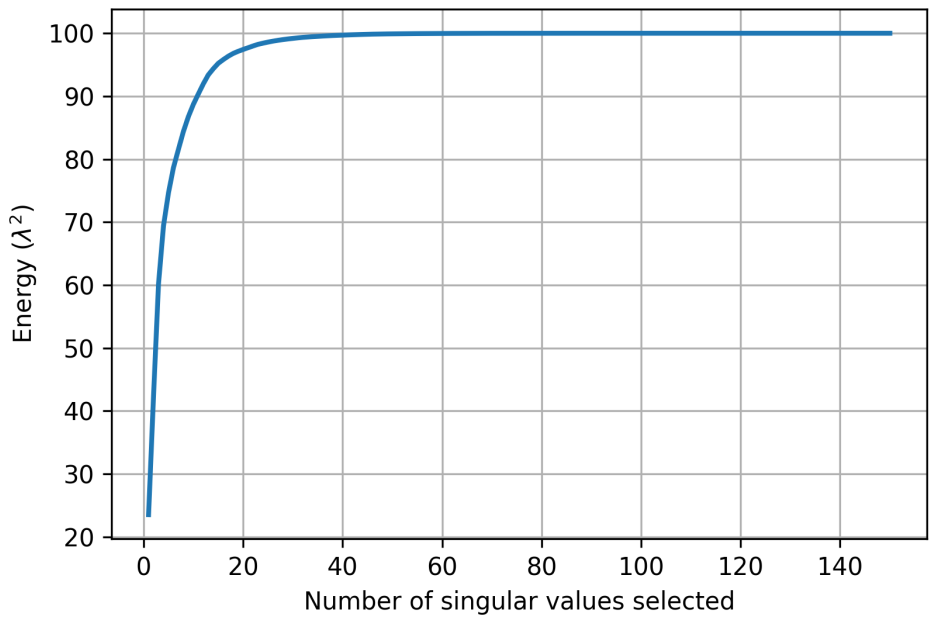
\includegraphics[width = 0.85\textwidth, height=70mm]{figures/energy_plot.png}
    \caption{Scatter energy verses number of singular values selected.}
    \label{energy plot}
\end{figure}

Figure \ref{energy plot} represents the scatter energy distribution against the number of singular values selected. By selecting the first ten principal components, it is possible to cover over $85\%$ of total scatter energy. Similarly, with 30 principal components, over $95\%$ of total energy is covered. Generally, the value of over $85\%$ is considered to be the good choice. Table \ref{scatter_energy} represents the exact number about the scatter energy distribution over the singular value selected.
\begin{table}
    \centering
    \begin{tabular}{|c|c|}
        \hline
        Singular values selected & Scatter energy ($\%$) \\\hline
         1 & 23.52\\
         2 & 42.48\\
         5 & 74.63\\
         10 & 88.70\\
         \textbf{20} & \textbf{97.42}\\
         30 & 99.17\\
         50 & 99.98\\ \hline
    \end{tabular}
    \caption{Singular value selected against scatter energy}
    \label{scatter_energy}
\end{table}

It is possible to capture over $97\%$ of total scatter energy by selecting the first 20 singular values, whereas selecting the first 30 principal components will capture over $99\%$ of total scatter energy. However, there is no significant improvement in the total scatter energy captured. Also, with the higher singular value selected, more will be the computational cost, which affects the convergence rate. So a singular value of 20 is considered to be a good choice. Also, the number of the singular value selected is analogous to the dimension of problem. By selecting the first 20 leading principal components, the entire dimension of problem is reduced from 125 (previous) to 20 (present). This is a significant improvement in terms of the convergence rate of the optimizer.  
\begin{figure}[!htbp]
    \centering
    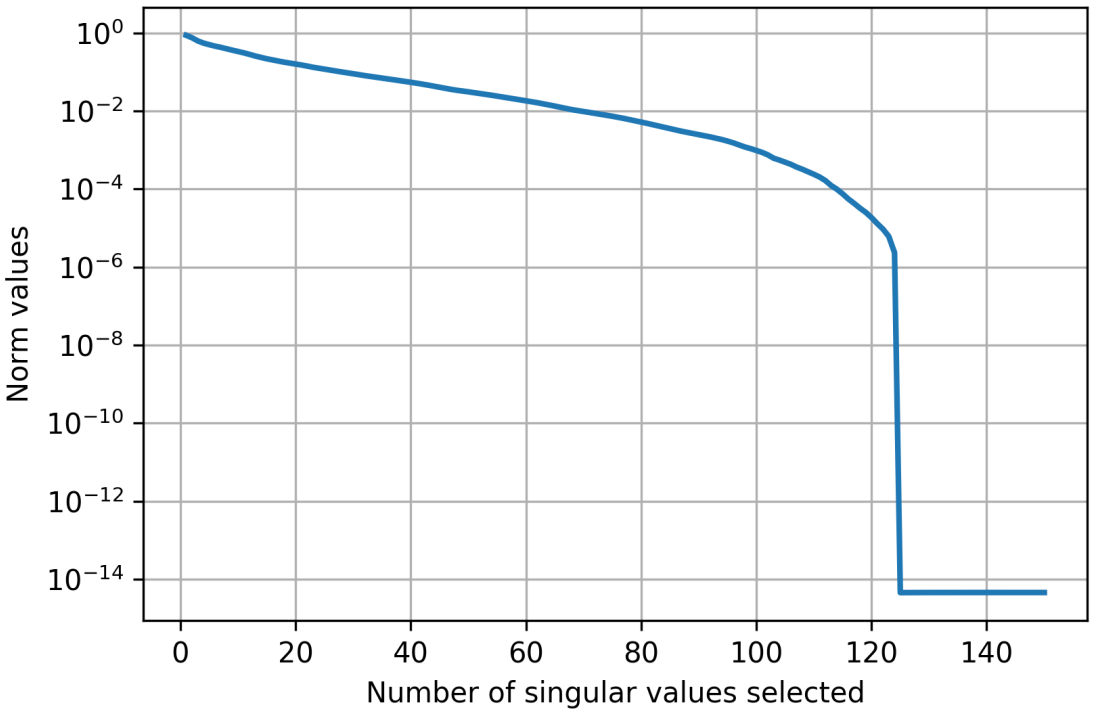
\includegraphics[width = 0.85\textwidth, height=70mm]{figures/norm_x_plot.png}
    \caption{Plot representing the norm value against the singular value selected.}
    \label{norm plot}
\end{figure}

Figure \ref{norm plot} represents the norm value calculated for various singular values selected. Y-axis represents the norm value which is calculated using equation \ref{Norm_value}.
\begin{equation}
    \text{Norm value} = \frac{norm (X - X^*)}{norm (X)}
    \label{Norm_value}
\end{equation}

where,\\
$X$ is the covariance matrix of a full size $(1000 \times 90000)$.\\
$X^*$ is the covariance matrix of a singular values selected.

For example, let $t$ be the number of leading principal components being selected. The matrix $X^*$ will be a matrix multiplication between $U_s$, $\Sigma_s$, and $V^T_s$. that is, $$X^* = U_s \Sigma_s V^T_s$$

where,\\
$U_s$ is the matrix consisting of first $t$ columns (1000 $\times$ $t$).\\
$\Sigma_s$ is the diagonal vector with $t$ elements ($t$ $\times$ $t$).\\
$V^T_s$ is the matrix with first $t$ rows ($t$ $\times$ 90000).

From figure \ref{norm plot}, it is observed that at the singular value of 20, the norm value obtained is of order $10^{-1}$, which is a good choice to proceed with the optimization. Further, at the singular value of 125, the graph drops vertically to $10^{-14}$, which is $\approx$ zero, indicates that if 125 singular values are selected, then $X=X^*$. This step confirms that the previous dimension was 125.

\section{Selecting design space}
After selecting the number of singular values to 20, evaluation of the matrix $U_s$ and $\Sigma_s$ is carried. let $A$ be a matrix such that $A = U_s \Sigma_s$. The matrix $A$ is of size $(1000 \times 20)$. Later, the maxima and minima of each column of $A$ are identified. If the maxima and minima values are the same in magnitude, then the design space is symmetric with the origin. Otherwise, select the smallest (by magnitude) among them and replace it with the previous one.

For example, if $a$ and $b$ are the maximum and minimum values of a given column, $|a|<|b|$, then chose $a$ as the extreme point and replace the previous design space to $(a, -a)$ and vice verse. The design space obtained in this work is appended in \ref{design space}. In all 20 dimensions (direction), the design space is made symmetric about the origin.

\section{Generating initial population}
After deciding the design space, the next step is to evaluate the wing surface coordinates. Based on the availability of computational power, a population size $(N)$ of 20 is chosen. Further, between individual design space, a set of random numbers of size equals to population size (in this work it will be 20) are generated. Each vector is named as target vector in optimization algorithm. This results in a matrix $A_g$ of size $20 \times 20$. The matrix $A_g$ is multiplied with $\Sigma_g$ and $V^T_g$ resulting in the matrix $X_g$ in equation \ref{svd_approx}.

\begin{equation}
   X_g = A_g \Sigma_g V^T_g
   \label{svd_approx}
\end{equation}

where,\\
$X_g$ is the covariance matrix representing the randomly generated wings.\\
$\sigma_g$ is the diagonal matrix containing the first 20 singular values.\\
$V^T_g$ is the matrix containing the first 20 rows of $V^T$.

Further, the obtained matrix $(X_g)$ is added to mean of error vectors $(\Bar{x})$, and the baseline geometry coordinates $(x^0)$ resulting in matrix $M$. In the present work, the matrix $M$ is of order $20 \times 90000$. Each row in $M$ represents the cartesian coordinates of the randomly generated wing and is arranged in the order $(x_1, y_1, z_1, ..., x_n, y_n, z_n)$. Each wing's coordinates are rearranged to the Plot3D format (*.x3d) and script to a file.

$$ M = x^0 + \bar{x} + X_g $$

$M$ is as called a reduced-order model.

The generated wing is imported to pointwise in the Plot3D format. Similarly, the principal modes of wings are generated and imported to pointwise. However, they did not depict any positive sense. For example, it was expected that the first principal mode would indicate the span property, thickness property, independently. Instead, the principal modes showed the mixed behavior of thickness, span, chord variation property. This leads to an insignificant conclusion towards wing behaviors. Figure \ref{svd_wing_1} to \ref{svd_wing_3} illustrates the wings generated after implementing the PCA. It is observed that the wing shape generated almost represents the wings those being generated after the FFD box implementation(fig \ref{wing1_iso}). More on this is explained in chapter \ref{results}.

\begin{figure}
    \centering
    \framebox{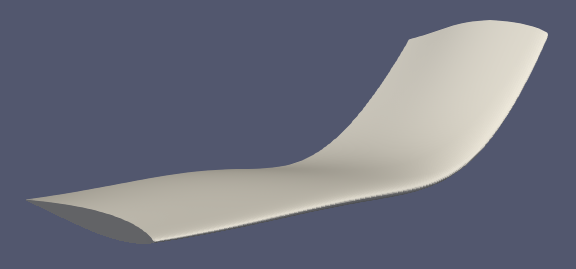
\includegraphics[width=0.95\textwidth, height=60mm]{figures/svdwing1.png}}
    \caption{General SVD wing 1.}
    \label{svd_wing_1}
\end{figure}

\begin{figure}
    \centering
    \framebox{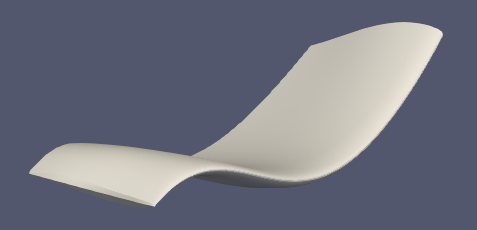
\includegraphics[width=0.95\textwidth, height=60mm]{figures/svdwing_2.png}}
    \caption{General SVD wing 2.}
    \label{svd_wing_2}
\end{figure}

\begin{figure}
    \centering
    \framebox{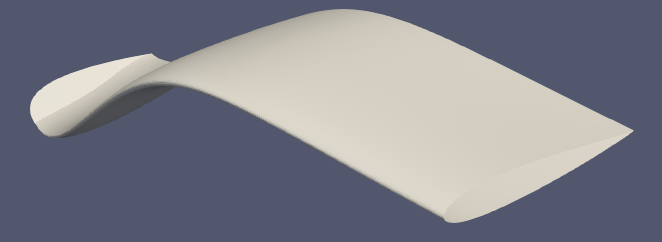
\includegraphics[width=0.95\textwidth, height=60mm]{figures/svdwing_3.png}}
    \caption{General SVD wing 3.}
    \label{svd_wing_3}
\end{figure}

\section{Implementing niching algorithm}
Several niching algorithms were implemented and tested successfully over the test functions. However, with the available time, it became possible to implement the fNRAND1 algorithm alone for multimodal optimization of the NACA0012 wing. A detailed explanation of the algorithm is presented in section \ref{fNRAND1_parallel_algorithm}. A fewer modification to the algorithm is made to make it fit the problem. These issues are highlighted, and the solution to mitigate them are discussed.  

The first step in implementing the algorithm is to construct the initial population of the wings. Initially, the population is randomly constructed, as mentioned above and the target vector is saved to python variable. The entire population is subjected individually for winglet creation. A glyph script is built, which imports the geometry (*.x3d) into pointwise and identifies the extreme coordinates wing tip section. 

To construct the winglet, a shoulder point of the curve is the first requirement. First, evaluate the average value of the extreme coordinates along chord and thickness direction, and along the span direction, the coordinates will be 2\% of the span length. With the help of shoulder point coordinates, the curve is constructed. Further, an unstructured mesh is generated from the wingtip section to the curve. Figure \ref{winglet} represents the winglet created at the wingtip section.

\begin{figure}[!htbp]
    \centering
    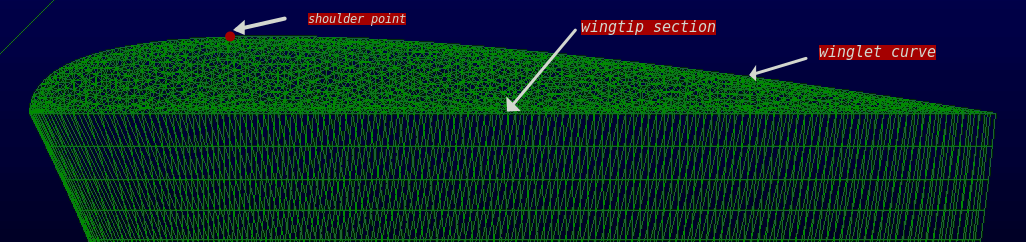
\includegraphics[scale=0.4]{figures/winglet_1.png}
    \caption{Winglet at wingtip section}
    \label{winglet}
\end{figure}

After completing the winglet section, the next approach is to generate a volume mesh over the entire wing surface. A box volume mesh of size 15 units (1 unit = 1 chord length of baseline wing) in all three directions is generated. Further details about the volume mesh and boundary conditions will be explained in chapter \ref{solver}. Once the volume mesh is generated and boundary conditions are applied, the mesh is exported in the SU2 format (*.su2). Each of these su2 files is subjected to function evaluations, which is SU2 simulation. Each simulation is considered as an individual job and subjected to different threads of the cluster. 

After the end of the simulation, the lift coefficient, drag coefficient, and moment coefficient about the chord direction are filtered from the file and subject to further evaluations. Proper coordination between the wing generation and mesh generation using pointwise and CFD simulations using SU2 solver is primarily managed by building a python code.

If any wing fails to create the volume mesh, the possible reason could be the presence of wing surface wrinkles. The better approach to resolve this issue is by regenerating the wing and subject it to generate the volume mesh. 

After generating the initial random wings, they are subjected to optimization cycles. A generation cycle of 50 and a population size of 20 is chosen. Mutation step contains a scaled vector addition of target vectors, resulting in a mutant vector. Later, the mutant vector is subjected to the crossover phase. For each element in the mutant vector, corresponding random value between 0 and 1 is generated and compared with the predefined value (crossover probability factor). After the end, a trial vector is obtained, and using this trail vector; wing surface coordinates are generated and script to a file. Further, this file is imported to pointwise using glyph script, and after creating winglet and volume mesh, it is export to SU2 solver. After completion of the CFD simulation, the required coefficients are extracted from the output file.

The moment coefficient constraint is satisfied using feasibility rules given by \cite{Deb}. Based on the fitness value, the target vector will get replaced by a trial vector. With the modified target vector, the generation cycles are continued for the remaining number of generation cycles. After each generation's end, the target vector is scripted to a file and is subjected to check for the existence of multimodality in a given design space. Specific details about how CFD simulation is carried and the ways to submit jobs are explained in chapter \ref{solver}.

All python codes and other related information can be found in \href{https://github.com/neelu065/M-Tech_project_code.git}{\underline{GitHub}}.